


\section{Experimental evaluation}\label{sec:exper}
We conducted an experimental evaluation of our algorithm and
compared its performances with those of other existing algorithm, both
exact~\citep{Brandes01} and approximate~\citep{BrandesP07,JacobKLPT05}.

\paragraph{Goals} 

The experiments are designed to study and compare the behavior of the proposed algorithm in terms of execution time and workload.
Specifically we study the scenario where the user gives as an input a ($\epsilon$,$\delta$) pair of guarantees that meet the quality criteria of the purpose and scale of the corresponding  graph.
We use two metrics in order to measure the amount of computations that the algorithms perform.
The first metric is the execution time, or \textit{time}, in seconds, the second metric is the number of edges that the algorithm touched/traversed, or \textit{touched edges}, during the execution.
The number of touched edges is a graph theoretic metric that does not depend on the specifications of the implementation environment and gives a perspective of the amount of work that the algorithm requires.
It is worth mentioning that we count an edge as many times as it is touched  during the execution of a given pair of guarantees, so we might count a single edge more than once.
The goal is to approximate the betweenness values of all the nodes so as to meet the given ($\epsilon$,$\delta$) guarantees in an efficient way for the  criteria time and touched edges.


\paragraph{Implementation and environment}
We implemented our algorithms, the one presented in~\citep{BrandesP07,JacobKLPT05}
%, and the linear scaling version from~\citep{GeisbergerSS08}GeisbergerSS08BrandesP07
 in C, by extending the implementation of the exact algorithm~\citep{Brandes01} contained in igraph~\citep{igraph}. 
 The implementations are engineered similarly, given that they are based on the
same subroutines for the computation of the shortest path (Dijkstra's algorithm
for weighted graphs, BFS for unweighted ones) and received similar amount of
optimizations. We exposed our implementations through Python 3.3.1, which was
used for running the simulations. We run the experiments on a quad-core AMD
Phenom\texttrademark II X4 955 Processor with 16GB of RAM, running Debian
\emph{wheezy} with a Linux kernel version 3.2.0.

\paragraph{Datasets} We used a number of datasets from the Stanford Large
Network Dataset Collection\footnote{\url{http://snap.stanford.edu/data/index.html}}. 
These are all real world networks including online social networks, communication (email)
networks, scientific citation and academic collaboration networks, road
networks, Amazon frequent co-purchased product networks, and more. 
We refer the reader to the SLNDC website for details about each dataset.



\begin{figure*}
\begin{minipage}[b]{0.5\linewidth}
\flushleft
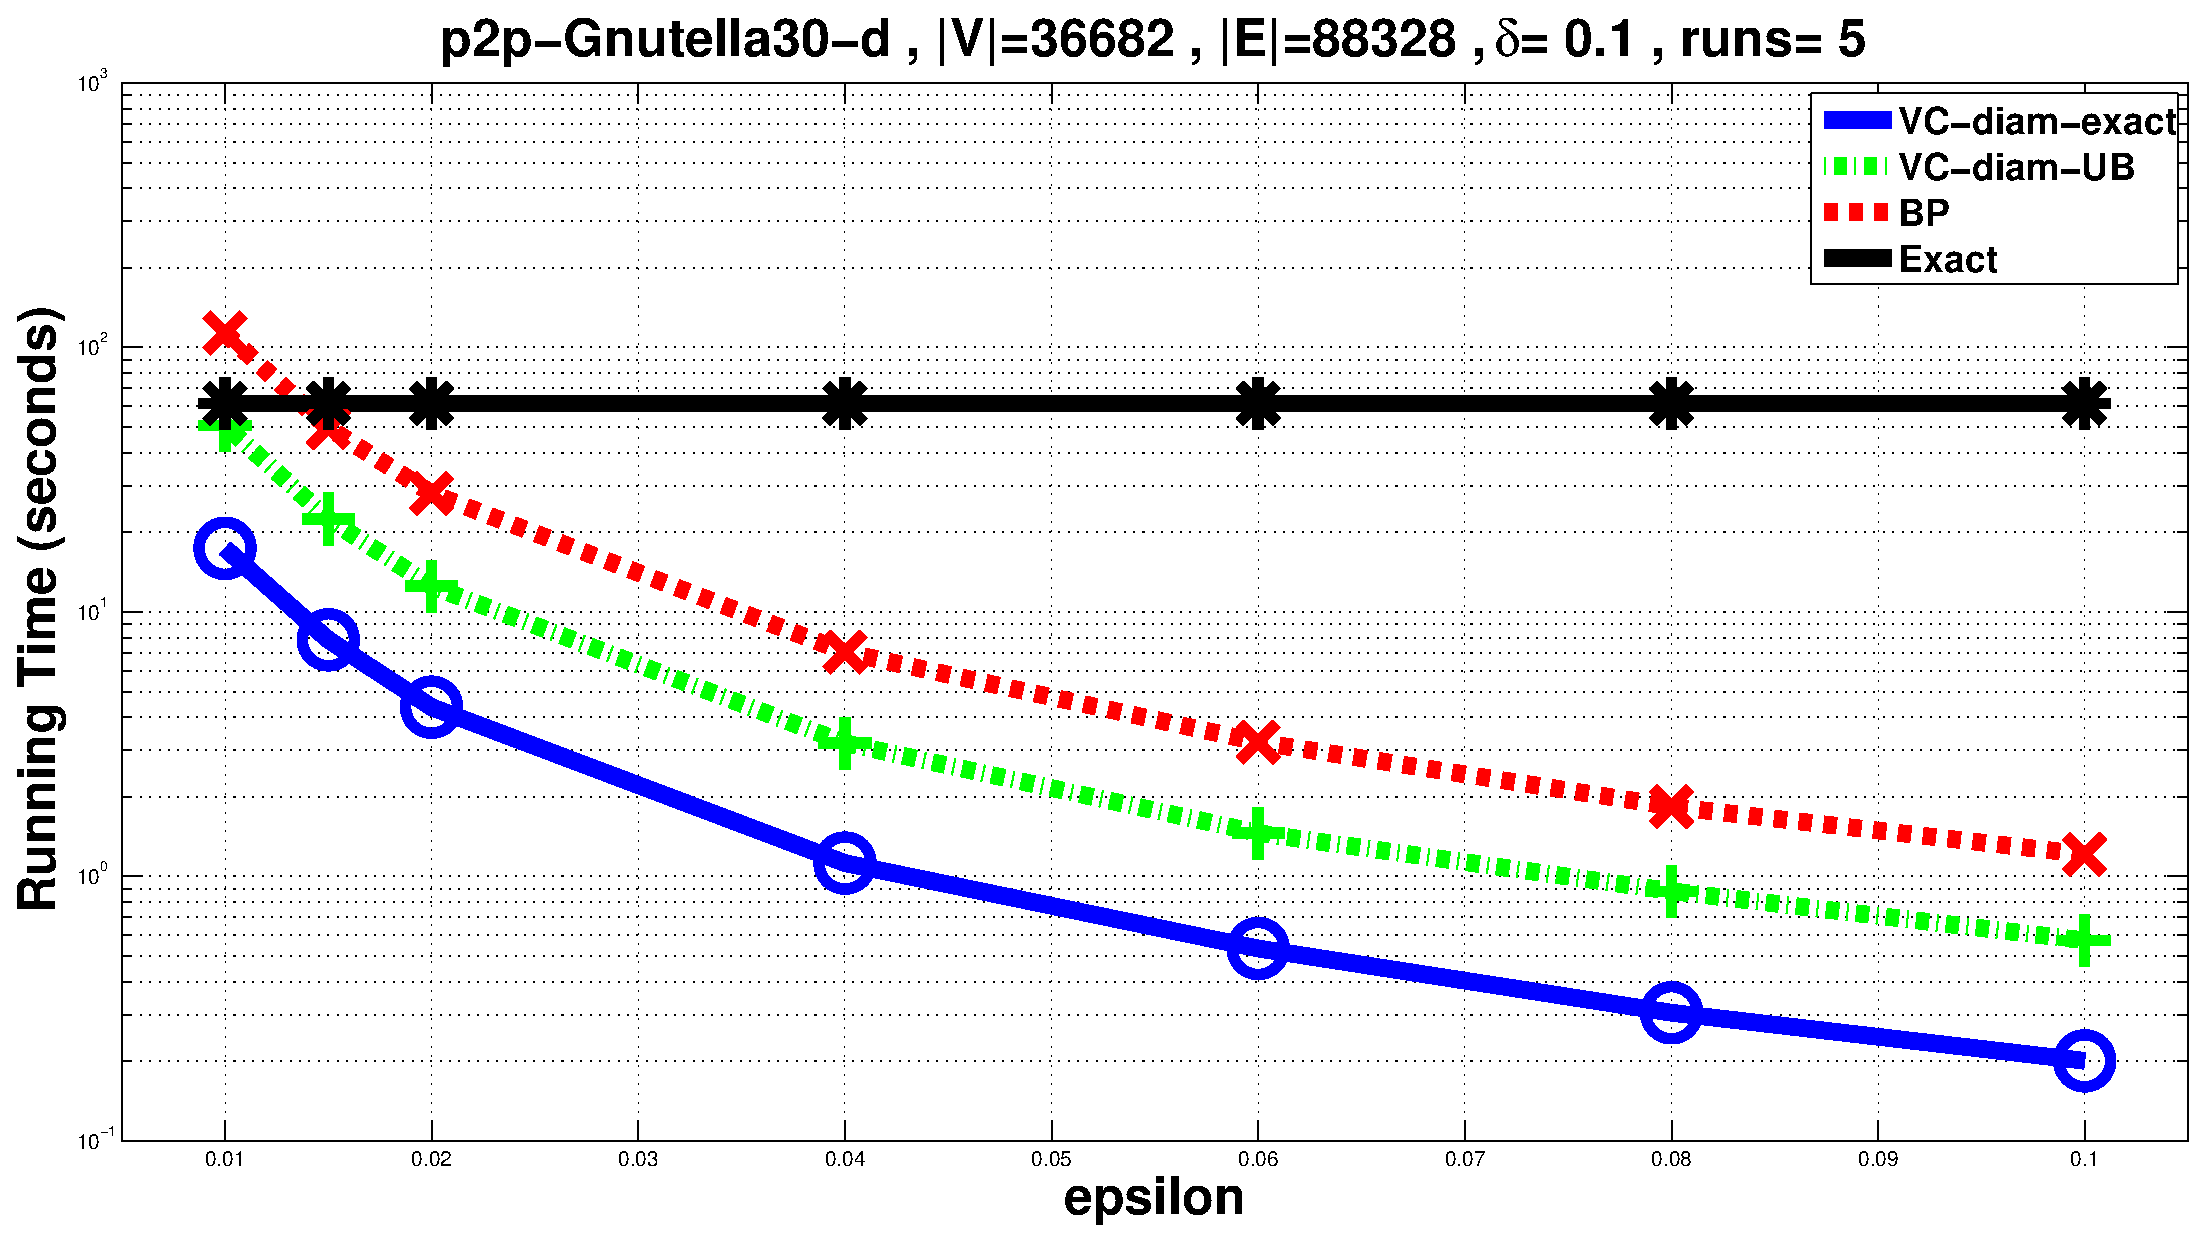
\includegraphics[width=3.8in, keepaspectratio]{p2p-Gnutella30-time.eps}
\caption{-} \label{fig:gnutella:time}
\end{minipage}%
\begin{minipage}[b]{0.5\linewidth}
\centering
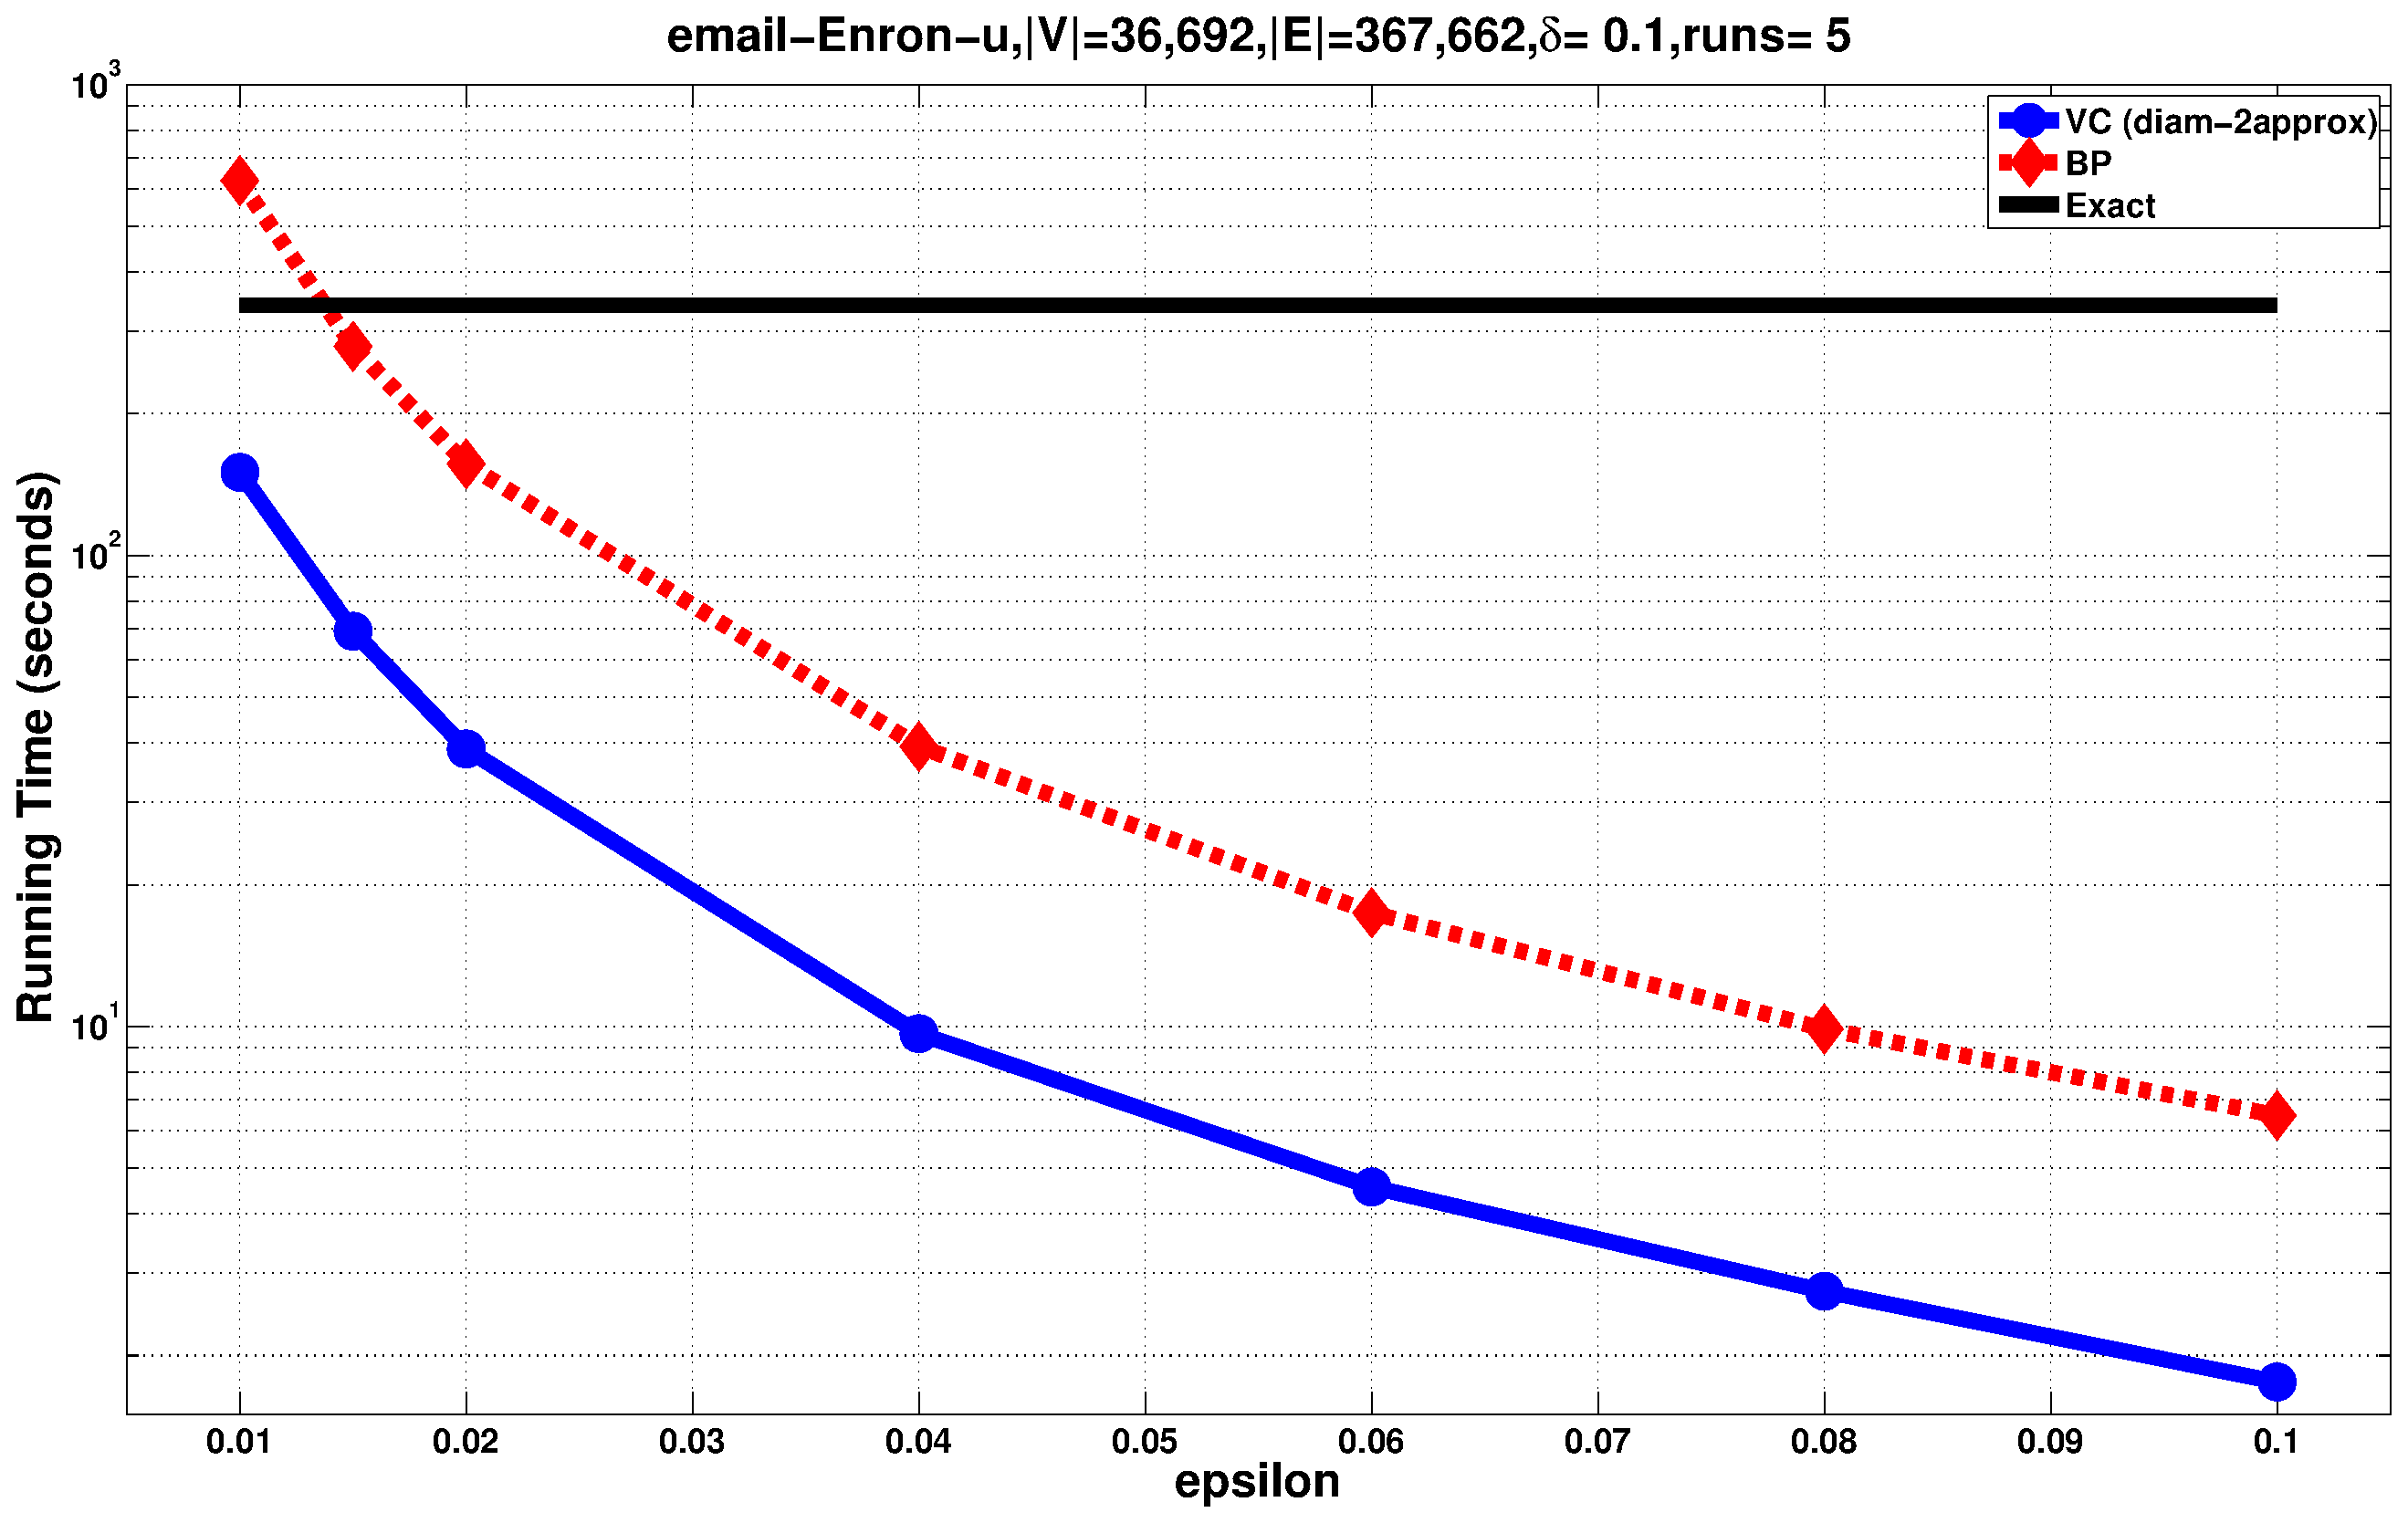
\includegraphics[width=3.8in, keepaspectratio]{email-Enron-time.eps}
\caption{-} \label{fig:email:time}
\end{minipage}
\end{figure*}
\begin{figure*}
\begin{minipage}[b]{0.5\linewidth}
\flushleft
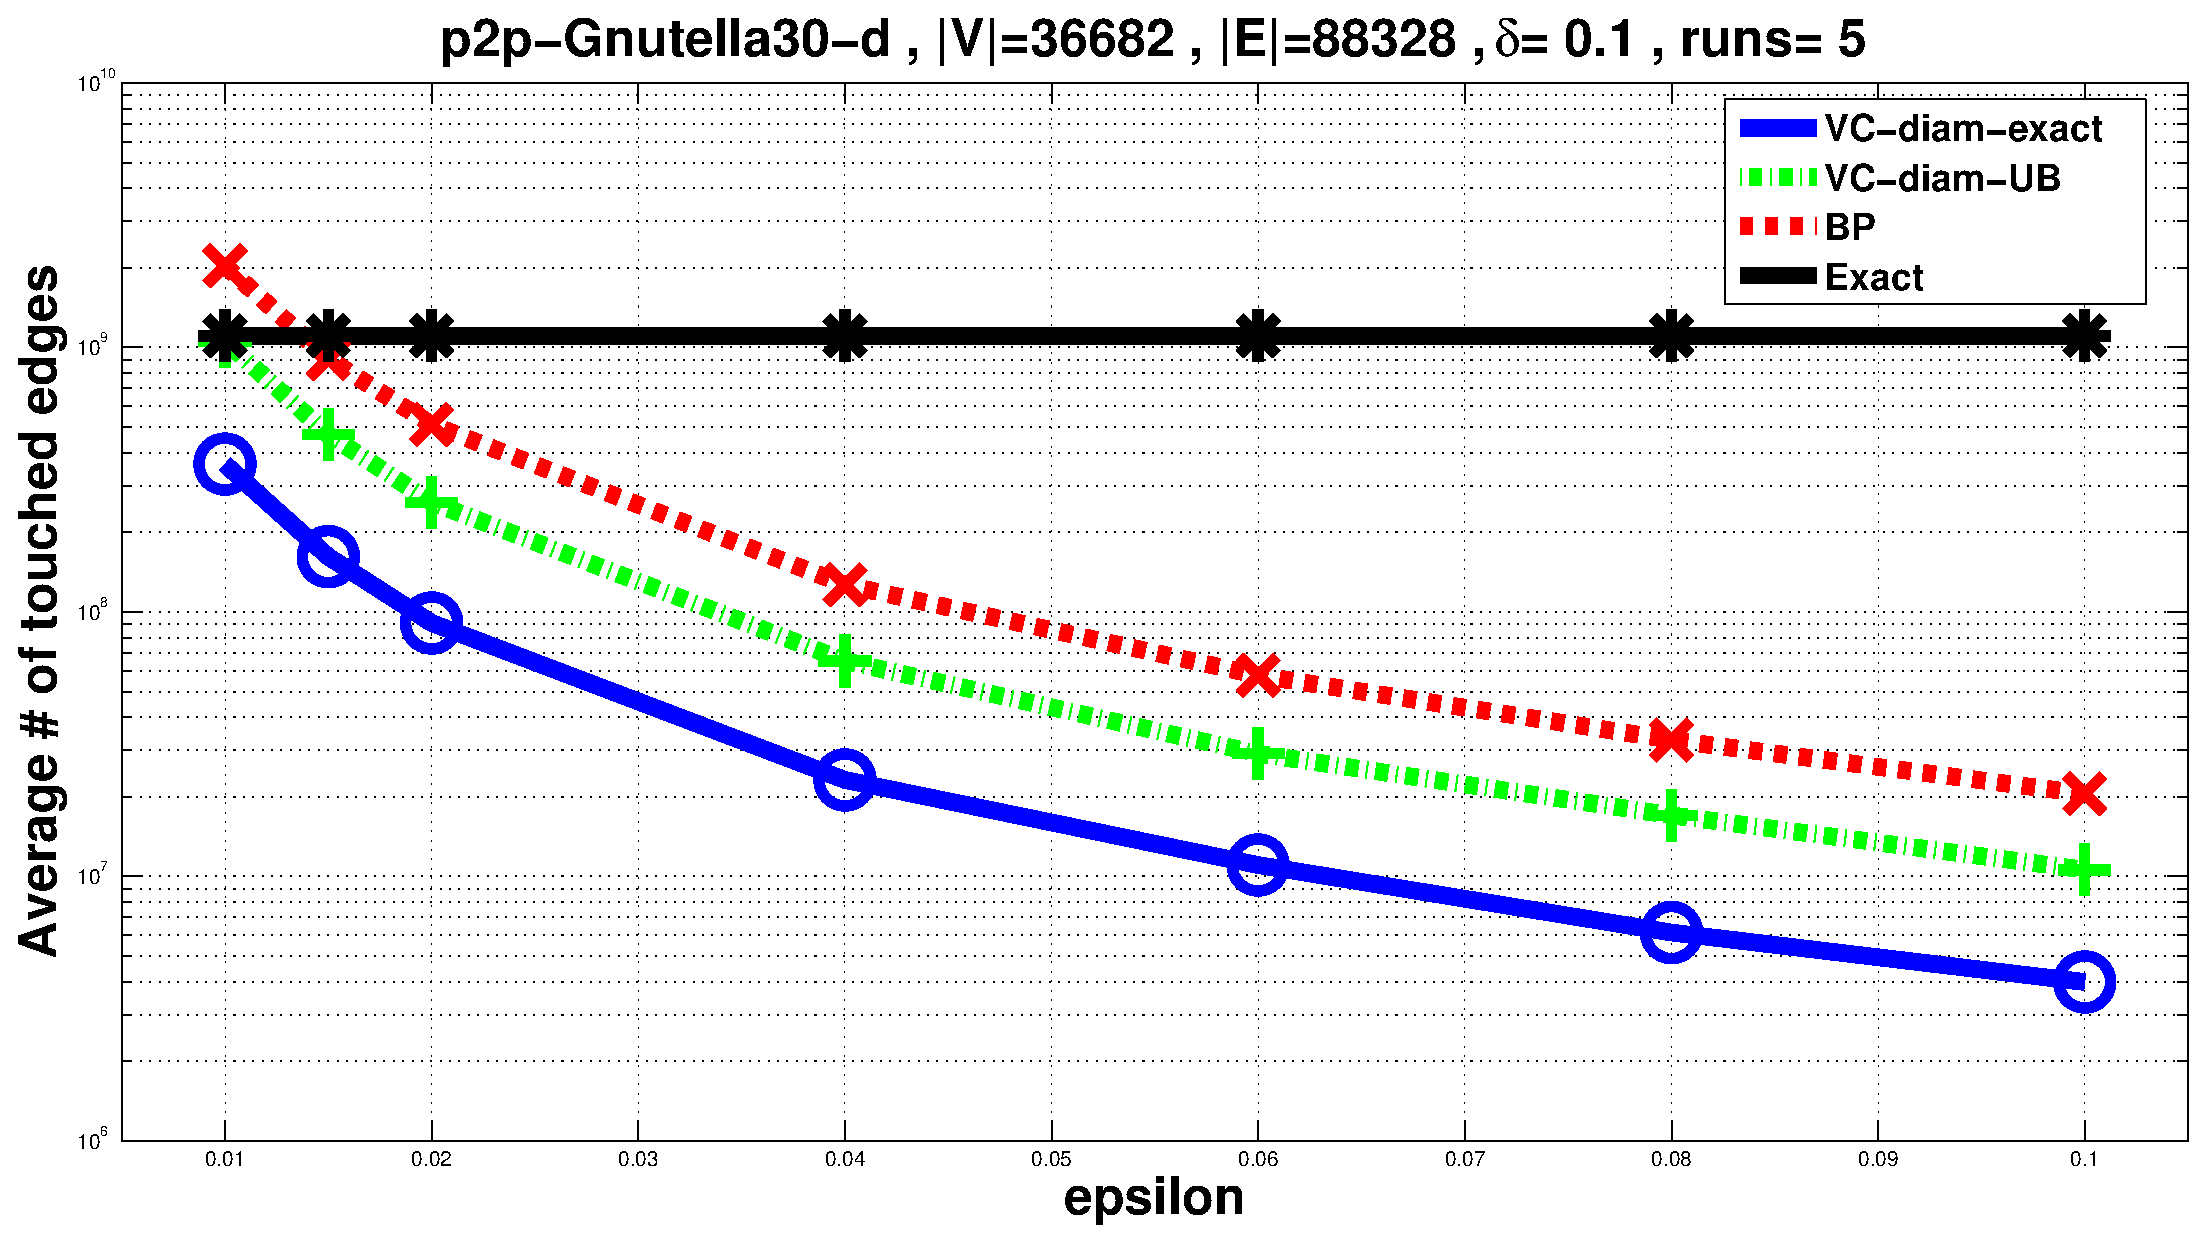
\includegraphics[width=3.8in, keepaspectratio]{p2p-Gnutella30-edges.eps}
\caption{-} \label{fig:gnutella:edges}
\end{minipage}%
\begin{minipage}[b]{0.5\linewidth}
\centering
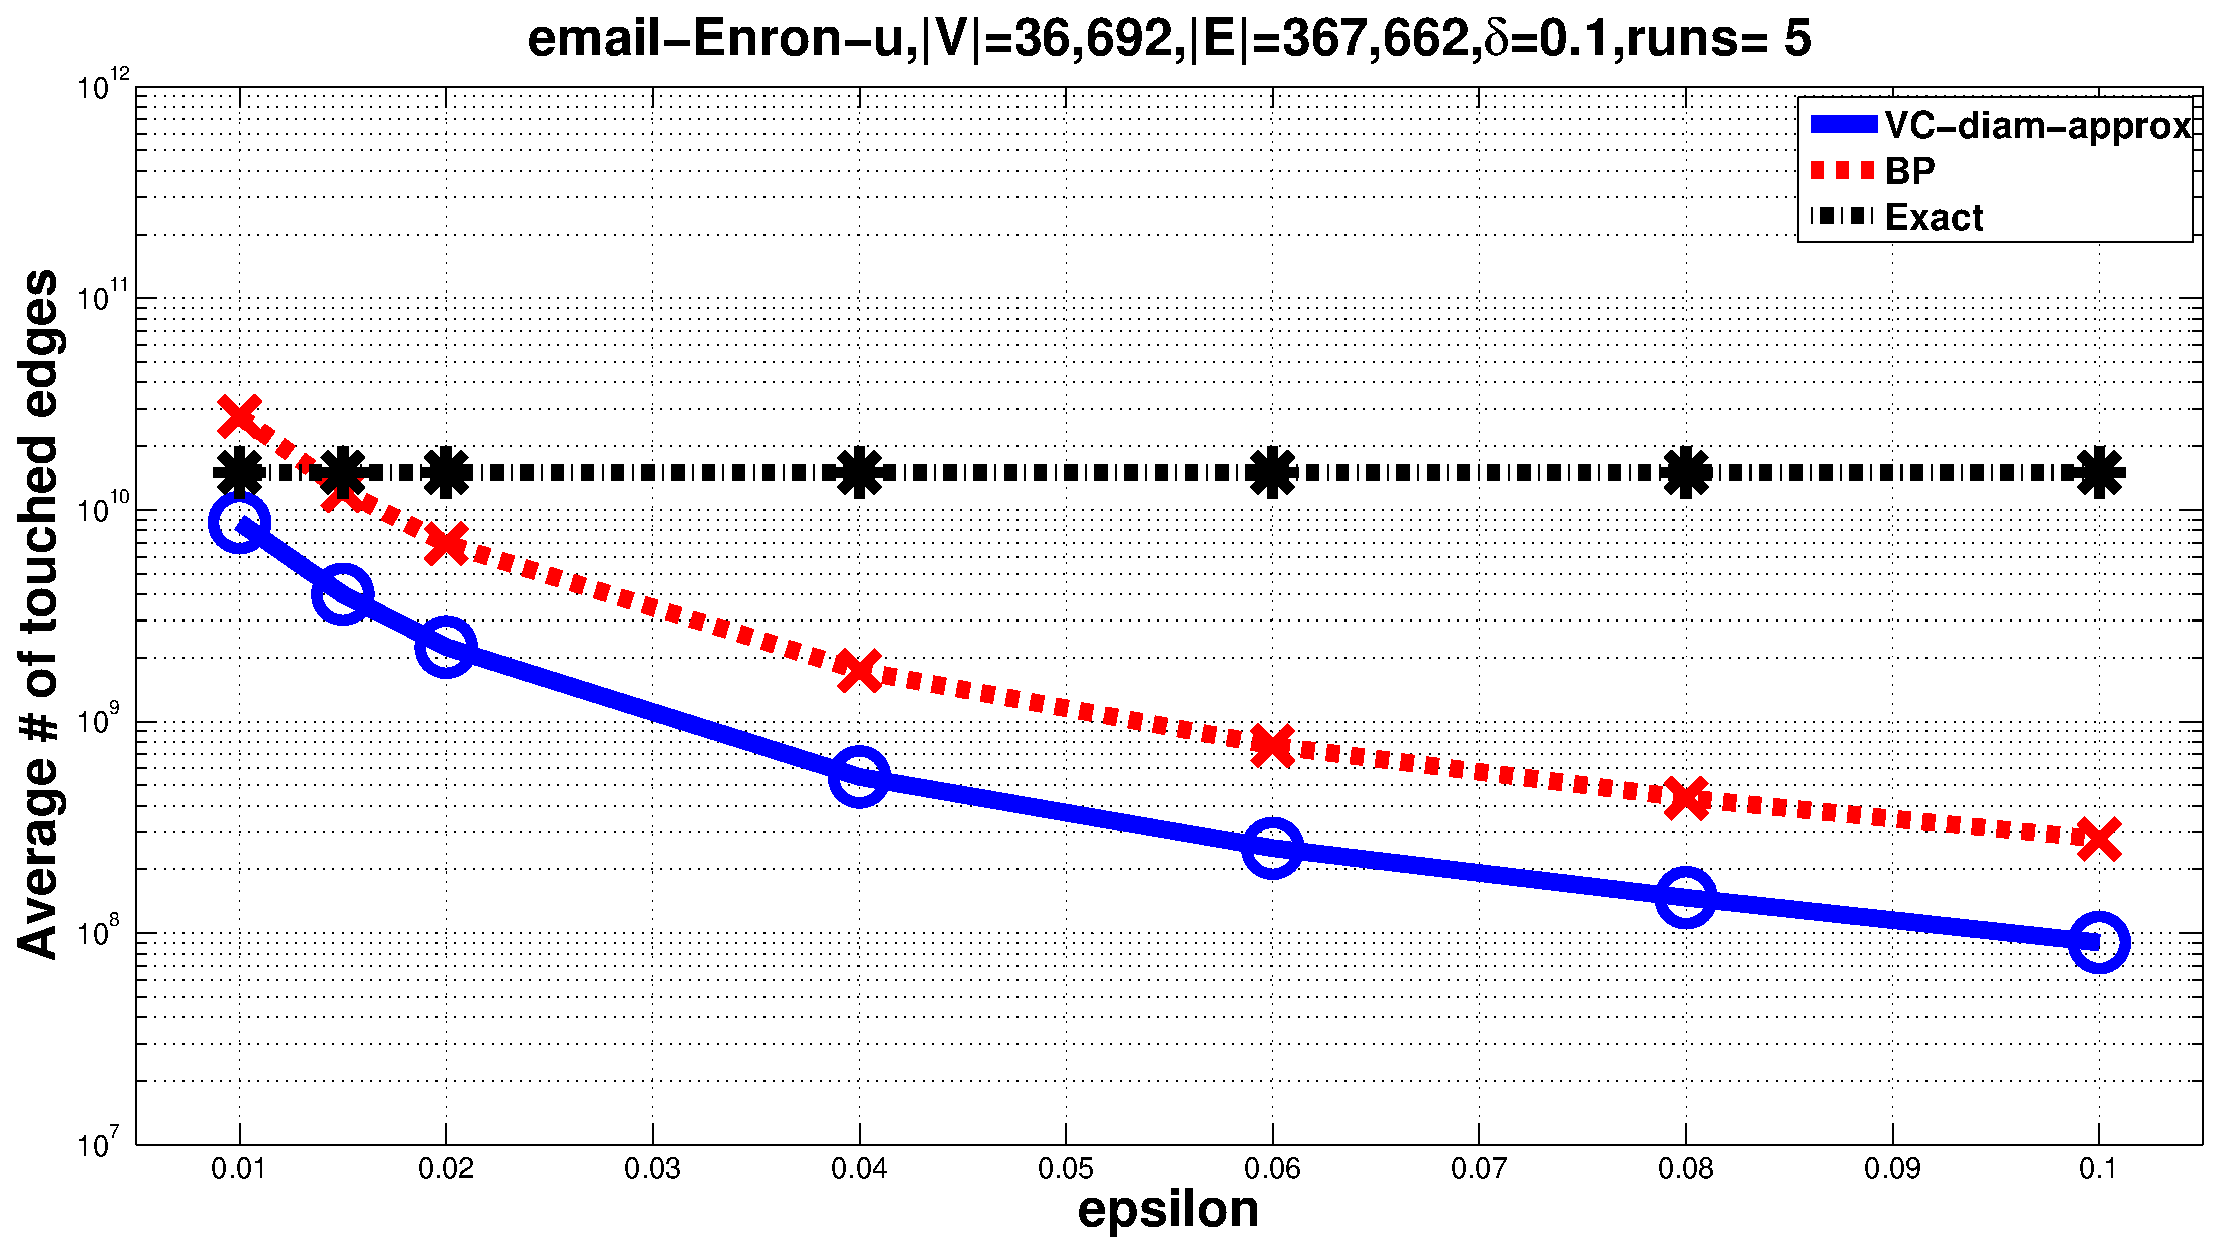
\includegraphics[width=3.8in, keepaspectratio]{email-Enron-edges.eps}
\caption{-} \label{fig:email:edges}
\end{minipage}
\end{figure*}



\begin{table*}[ht]
%\caption{Experiments on Undirected Graphs} % title of Table
\centering % used for centering table
\begin{tabular}{|c c c c |c c |c  c |} % centered columns (5 columns)
\hline\hline %inserts double horizontal lines
Graph & Node & Edges & Diameter  & \multicolumn{2}{|c|}{$\frac{\epsilon\mbox{-Edges-BP}}{ \epsilon\mbox{-Edges-VC}}$} & \multicolumn{2}{c|}{$\frac{\epsilon\mbox{-Time-BP}}{\epsilon\mbox{-Time-VC}}$}\\ [0.5ex] % inserts table 
\hline
&  &  & &\multicolumn{4}{|c|}{diam-2-approx} \\
\hline
&  &  & & min & max & min & max\\
%heading
\hline % inserts single horizontal line
%\multirow{6}{35mm}{\begin{sideways}\parbox{15mm}{Undirected\\ diam-approx}\end{sideways}}\\
oregon1-010331 & 10,670 & 22,002 & 9 & 3.69 & 3.73 & 4.39 & 4.75\\  % [1ex] adds vertical space
oregon1-010526 & 11,174 & 23,409 & 10 &  3.53 & 3.74 & 4.26 & 4.73 \\
ca-HepPh & 12,008 & 237,010 & 13  & 2.43 & 2.49 & 3.06 & 3.33\\
ca-AstroPh & 18,772 & 396,160  & 14  & 2.81 & 2.95 & 3.26 & 3.76\\
ca-CondMat & 23,133 & 186,936 & 15  & 3.24 & 3.26 & 3.75 & 4.08\\
email-Enron & 36,692 & 421,578 & 12  & 2.98 & 3.18 & 3.60 & 4.16\\[1ex] % inserting body of the table
\hline %inserts single line
\end{tabular}
\caption{
%For each graph efficiency measures generated  for a given input  as the average of 5 runs for a  pair of given values $\epsilon,\delta$.
%The value of $\delta$ was 0.1 and $\epsilon$ took values 0.01, 0.015, 0.02, 0.04, 0.06, 0.08, 0.1.
%Among the 6 data points that produced with varied $\epsilon$ we present the minimum and maximum ratios of the Brandeis-Pitch method over VC-dimension method for the number of touched edges during the execution and time.
%In both undirected and directed graphs the exact value of the diameter was used. For each ($\epsilon,\delta$) the experiment was repeated 5 times and the average was recorded.
}
\label{table:expUndir} % is used to refer this table in the text
\end{table*}


\begin{table*}[ht]
%\caption{Experiments on Directed Graphs} % title of Table
\centering % used for centering table
\begin{tabular}{|c c c c | c c | c c | c c | c c | c c | c c|} % centered columns (5 columns)
\hline\hline %inserts double horizontal lines
Graph & Node & Edges & Diameter  & \multicolumn{2}{|c|}{$\frac{\epsilon\mbox{-Edges-BP}}{ \epsilon\mbox{-Edges-VC}}$} & \multicolumn{2}{c|}{$\frac{\epsilon\mbox{-Time-BP}}{\epsilon\mbox{-Time-VC}}$} & \multicolumn{2}{c|}{$\frac{\epsilon\mbox{-Edges-BP}}{ \epsilon\mbox{-Edges-VC}}$} & \multicolumn{2}{c|}{$\frac{\epsilon\mbox{-Time-BP}}{\epsilon\mbox{-Time-VC}}$} & \multicolumn{2}{c|}{$\frac{\epsilon\mbox{-Edges-BP}}{ \epsilon\mbox{-Edges-VC}}$} & \multicolumn{2}{c|}{$\frac{\epsilon\mbox{-Time-BP}}{\epsilon\mbox{-Time-VC}}$}\\ [0.5ex] % inserts table 
\hline
&  &  & &\multicolumn{4}{|c|}{diam-exact}  &  \multicolumn{4}{c|}{diam-UB} & \multicolumn{4}{c|}{Top-K}\\
%heading
\hline % inserts single horizontal line
&  &  & &min & max & min & max&min & max & min & max &min & max & min & max\\
\hline % inserts single horizontal line
%\multirow{6}{13mm}{\begin{sideways}\parbox{15mm}{Directed}\end{sideways}}\\
wiki-Vote & 7,115 & 103,689  & 7 & 2.99 & 3.10 & 3.35 & 3.69 & 1.04 & 1.06 &1.05 & 1.27 & - & - & - & -\\
p2p-Gnutella25 & 22,687 & 54,705 & 11 & 5.02 & 5.46 & 5.45 & 5.78 & 1.85& 1.94& 1.94 & 2.09 & - & - & - &-\\
cit-HepTh & 27,770 & 352,807 & 14  & 2.71 & 2.86 & 3.58 & 3.83 & 1.17 & 1.21 & 1.39 & 1.61 & - & -  & - & -\\
cit-HepPh & 34,546 & 421,578 & 12 & 3.51 & 3.68 & 4.91 & 5.01 & 1.20 & 1.25& 1.60 & 1.71 & - & -  &-  &-\\ % inserting body of the table
p2p-Gnutella30 & 36,682 & 88,328 & 10  & 5.33 & 5.63 & 5.02 & 5.46 & 1.92 & 1.99 & 2.08 & 2.22 & - & - & - & -\\
soc-Epinions1 & 75,879 & 508,837 & 13  & 3.06&  3.11 & 4.20 & 4.25 & 1.00 & 1.03 & 1.35 & 1.38 & - &  - & - & -\\ [1ex] % [1ex] adds vertical space
\hline %inserts single line
\end{tabular}
\caption{
%For each graph efficiency measures generated  for a given input  as the average of 5 runs for a  pair of given values $\epsilon,\delta$.
%The value of $\delta$ was 0.1 and $\epsilon$ took values 0.01, 0.015, 0.02, 0.04, 0.06, 0.08, 0.1.
%Among the 6 data points that produced with varied $\epsilon$ we present the minimum and maximum ratios of the Brandeis-Pitch method over VC-dimension method for the number of touched edges during the execution and time.
%In both undirected and directed graphs the exact value of the diameter was used. For each ($\epsilon,\delta$) the experiment was repeated 5 times and the average was recorded.
}
\label{table:expDir} % is used to refer this table in the text
\end{table*}

\subsection{Runtime evaluation}\label{sec:runtime}
The approximation algorithms take a value $\epsilon$ and a value $\delta$ and compute the sample size accordingly.
For our experiments we used $\delta=0.1$, while $\epsilon$ takes the following values  0.01, 0.015, 0.02, 0.04, 0.06, 0.08, 0.1. 
For each $(\epsilon,\delta)$ pair we run the experiment 5 times and we computed the average number of touched edges as well as the average running time.

The algorithm proposed in \cite{GeisbergerSS08} follows the same sampling approach as \cite{BrandesP07}.
But they differ on the way they update the estimated betweenness.
Therefore the running time and the number of touched edges that algorithm \cite{GeisbergerSS08} requires is the same as \cite{BrandesP07} (the quality of the solution though in \cite{GeisbergerSS08} is superior of the Brandes et al.\cite{BrandesP07} according to the experiments of the authors).
In our plots we present the performance of \cite{BrandesP07} given that the two algorithms behave the same in the two metrics that we are interested in.


As we discussed in the previous sections the number of samples that the proposed algorithm requires depends on the diameter of the graph.
For the computation of the diameter in case of undirected graphs we used the 2-approximation algorithm that we briefly described. 
In Table \ref{table:expUndir} we can see see the results from the comparison of the proposed algorithm with the Brandeis-Pitch(or BP) algorithm on undirected graphs.
For each of the 7 pairs of ($\epsilon,\delta$) we present the minimum and maximum ratio of the average touched edges of BP over VC, as well as the minimum and maximum ratio of the average running time of BP over VC.
As it can be seen from this table the proposed algorithm performs significantly faster, more than 300\%, in both measures.
In Table \ref{table:expDir} we compare the algorithms on a set of directed graphs.
As in the case of the undirected graphs, we present the minimum and maximum ratios among the seven ($\epsilon,\delta$) pairs for the corresponding measures.
We computed the number of samples using both the exact value of the diameter (indicated as diam-exact) as well as the trivial upper bound $|V|-1$ of the diameter (indicated as diam-UB).
From the table we can see that the value for diameter that we consider in the case of diam-UB is at least a thousand times greater than the actual value, which translates in a significant increase of the number of samples.
But even in the case of this crude diameter approximation (diam-UB), the proposed algorithm performs uniformly faster than \cite{BrandesP07}.
In the case where the exact value of the diameter was used, we can see that our algorithm meets the approximation guarantees 3 to 5 times faster than  \cite{BrandesP07}.
 \XXX-(COMMENT ON THE RELATION TOPOLOGY-SPEED)




In Figure \ref{fig:gnutella:time} we study the directed graph p2p-Gnutella30 and we present the measurements of the average running time of the algorithms in a logarithmic scale .
The proposed algorithm requires significantly less time than the Brandes algorithm.
The diam-UB and the diam-exact can be seen as the two extremes for the performance of our algorithm in terms of time.
In the case of the diam-exact we have as few samples as possible since we use the exact value of the diameter, whereas in the case of diam-UB we have as many samples as possibles since we use the worst case diameter of the graph (that is when the graph has a hamiltonian path).
In Figure \ref{fig:email:time} we study the average running time of the algorithms for the undirected graph email-Enron.
In this case the proposed algorithm not only to performs better but also scales better than the Brandes.
For the computation of the sample size we use the 2-approximation algorithm which is enough since what we really use for the computation of sample size is the the logarithm of the diameter.
In Figures \ref{fig:gnutella:edges} and \ref{fig:email:edges}, we study the average number of touched edges for the case of the directed graph p2p-Gnutella30 and of the undirected graph email-Enron, respectively.
The proposed algorithm outperforms both the Brandes and the exact algorithm in this measure too.


From the above Figures and Tables we see that for a given pair of guarantees ($\epsilon,\delta$) the proposed algorithm is faster(at least 3x speedup in case of exact diameter on the tested graphs) and requires less amount of work(at least 3x speed up on the tested graphs).
The reason is twofold, with our technique A) we use a significantly smaller amount of samples and B) only in the worst case we do the same amount of computations per sample as the state of the art.
Our proposed algorithm needs to find the shortest path between a sampled pair of nodes whereas in both the algorithms \citation{GeisbergerSS08,BrandesP07} we need to compute the shortest paths between a sampled source and all the rest of the nodes.





\subsection{Accuracy evaluation}\label{sec:accuracy}

\begin{figure*}
\begin{minipage}[b]{0.5\linewidth}
\flushleft
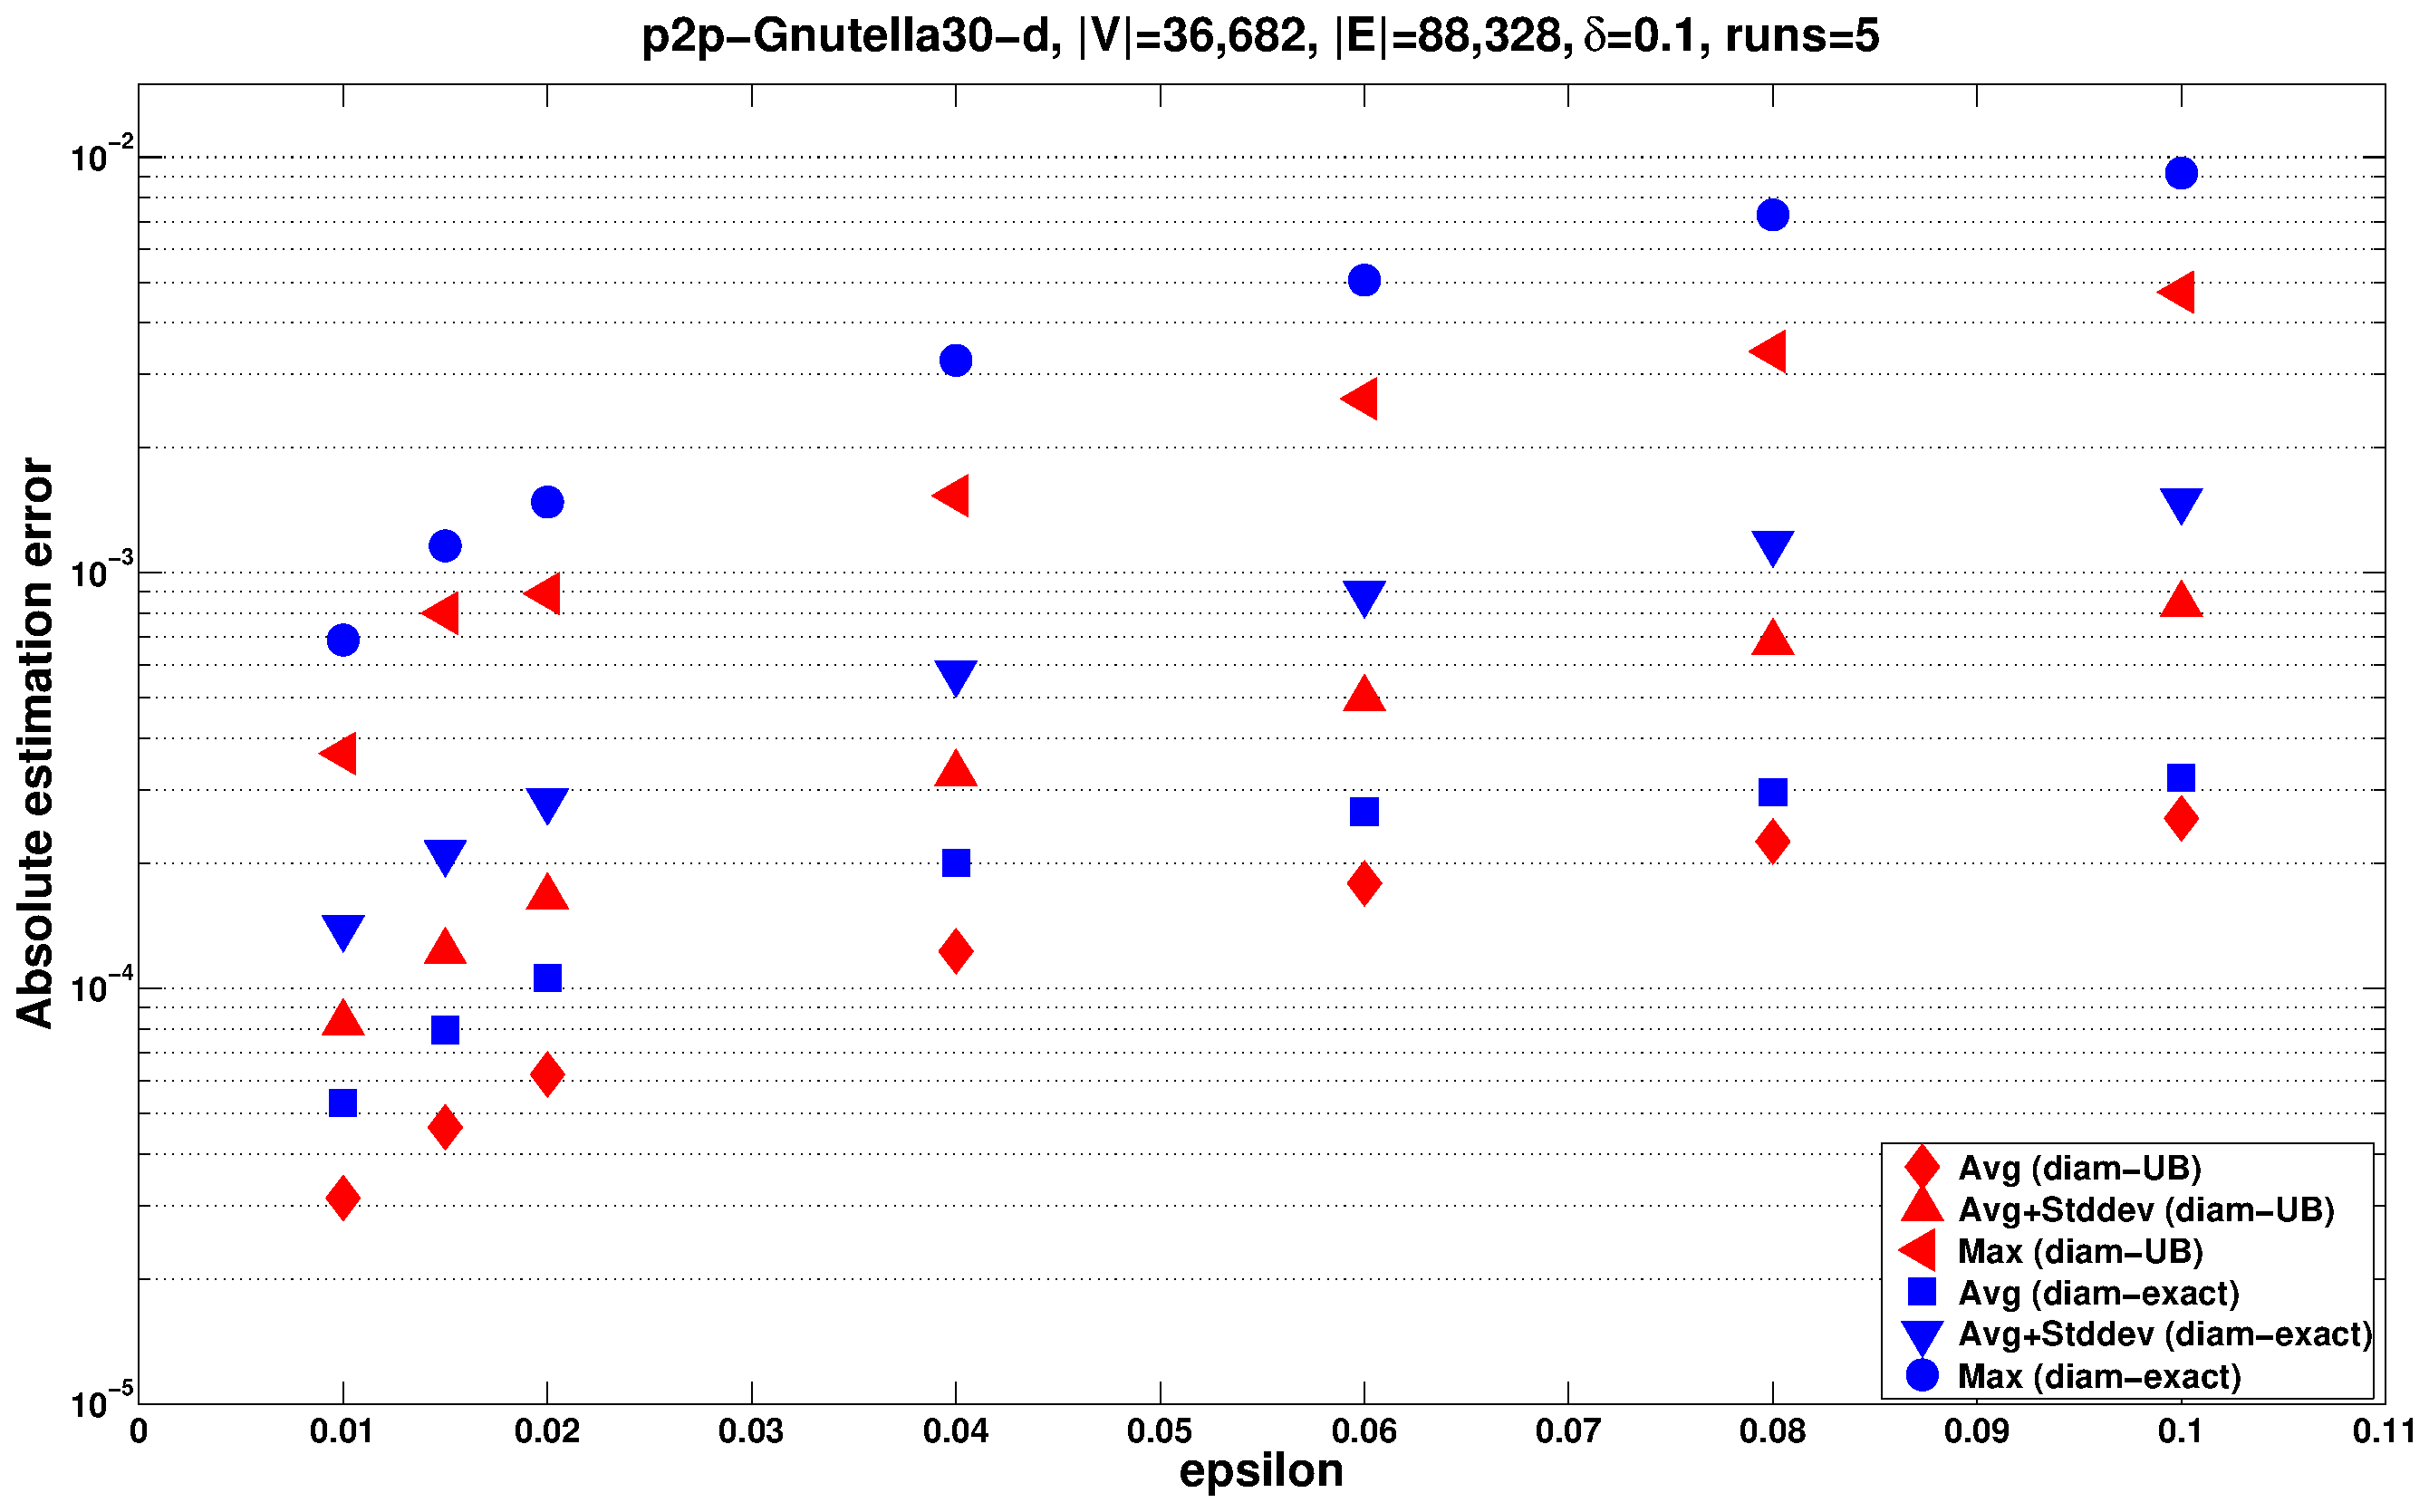
\includegraphics[width=3.8in, keepaspectratio]{p2p-Gnutella30-error.eps}
\caption{-} \label{fig:gnutella:error}
\end{minipage}%
\begin{minipage}[b]{0.5\linewidth}
\centering
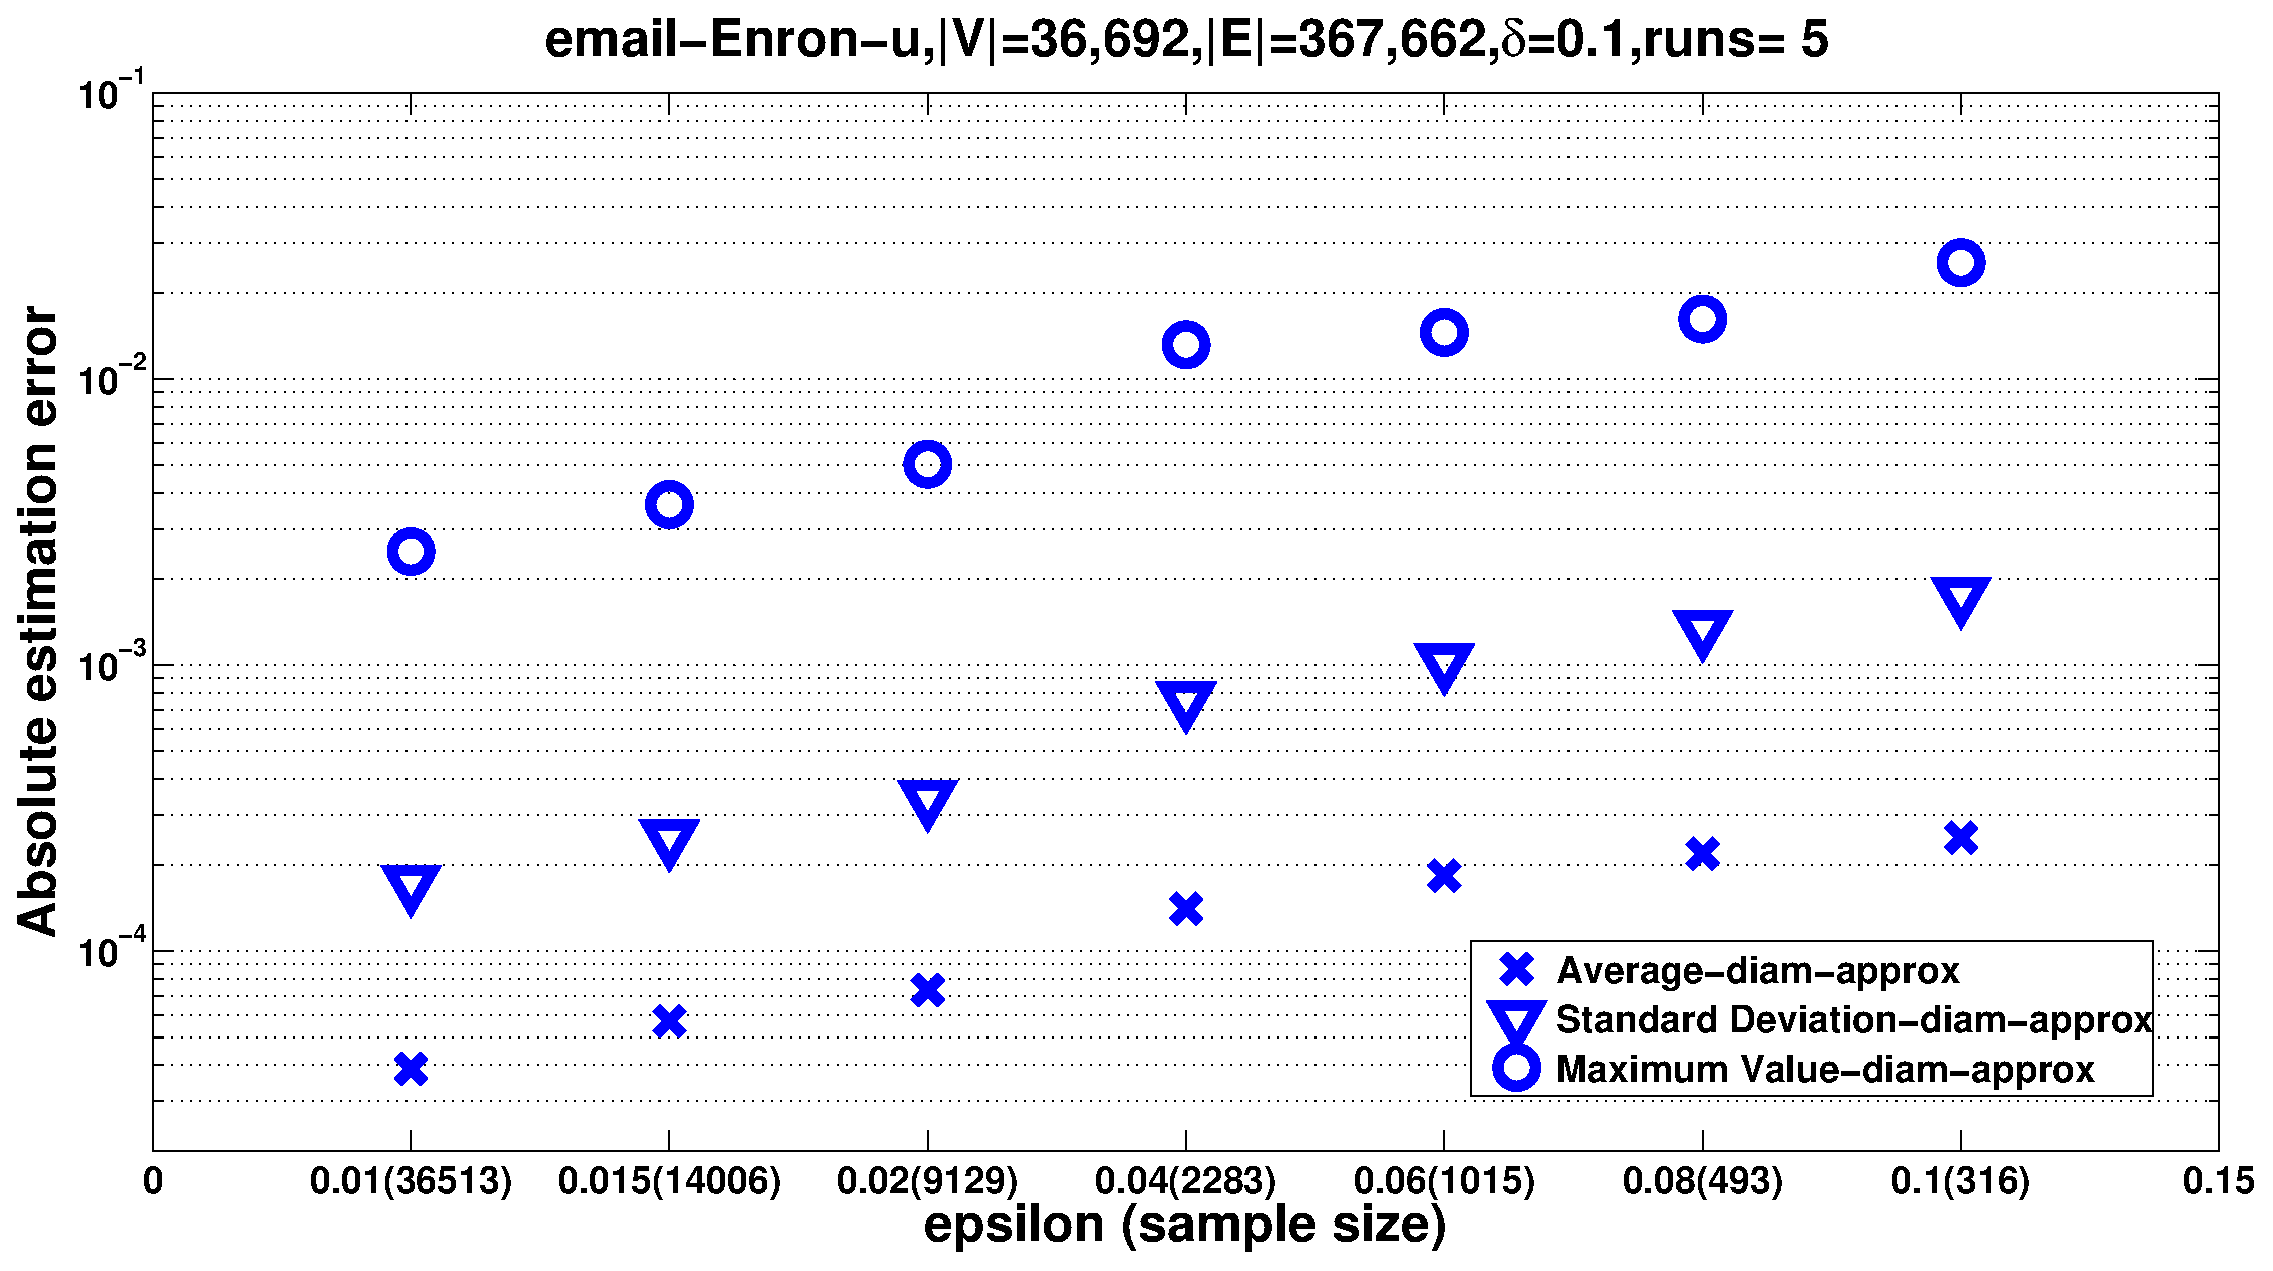
\includegraphics[width=3.8in, keepaspectratio]{email-Enron-error.eps}
\caption{-} \label{fig:email:error}
\end{minipage}
\end{figure*}
In Figure \ref{fig:gnutella:error} \ref{fig:email:error}

